\section{Rectificador}
La rectificación es el proceso de convertir una forma de onda de corriente
alterna en una forma de onda de corriente continua (en este caso, variable) que
tiene una sola polaridad.

\subsection{Media onda}
Considerando el circuito de la \textbf{figura~\ref{circuito02}}, se aprecia un
bucle en serie que consiste en una fuente de onda sinusoidal conectada a un
transformador; desde el transformador se conecta un diodo \textbf{1N4007} y una
resistencia de $10[\text{k}\Omega]$ que cumple la función de carga.

\begin{figure}[!h]
\centering
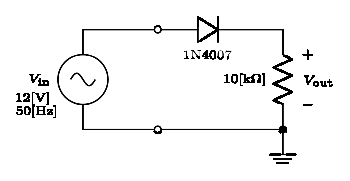
\includegraphics[scale=1.1]{diagramas/02.media_onda1.eps}
\caption{Rectificador de media onda.}
\label{circuito02}
\end{figure}

Para los valores positivos del voltaje de entrada, el diodo estará polarizado
directamente, por tanto la señal de entrada caerá a través de la resistencia de
carga; mientras que con los valores negativos del voltaje de entrada, hará que
el diodo este polarizado inversamente y por tanto no circulará corriente a
través de la carga.

\subsubsection{Simulación}
Se utilizó el software \emph{Quite Universal Circuit Simulator.} versión 23.3.1
para la simulación del rectificador de media onda, este puede verse en la
\textbf{figura~\ref{simulacion02}}.

\begin{figure}[!h]
\centering
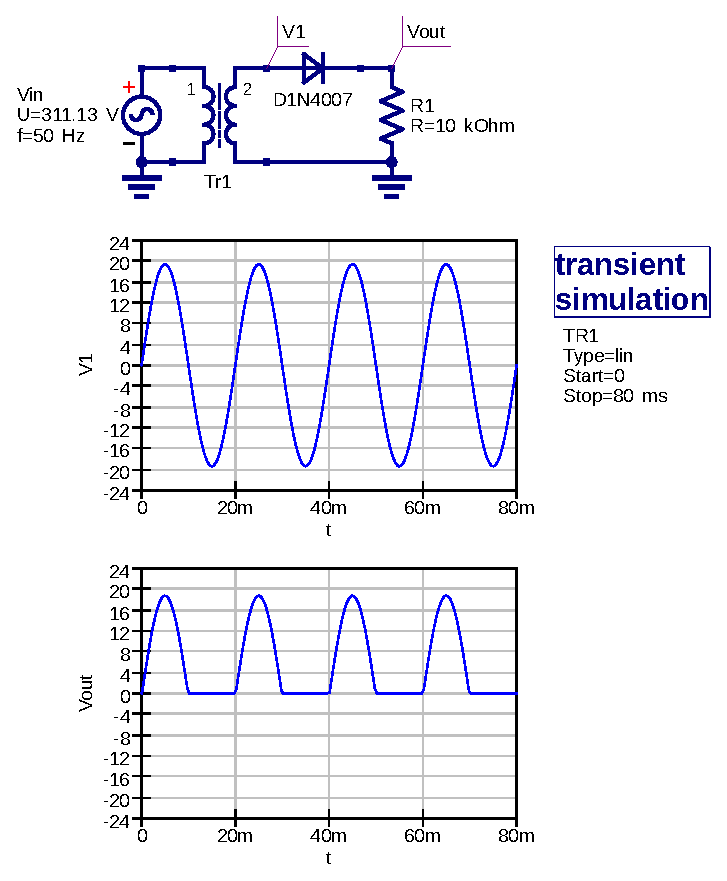
\includegraphics[scale=0.75]{simulacion/02.media_onda1.eps}
\caption{Simulación del rectificador de media onda.}
\label{simulacion02}
\end{figure}

\subsubsection{Laboratorio}
Se presenta el rectificador de media onda armado en laboratorio y su medición
de voltaje de salida en la carga, en la \textbf{figura~\ref{laboratorio04}}.

\begin{figure}[!h]
\centering
\includegraphics[scale=0.34]{fotos/02.media_onda1.eps}
\caption{Rectificador de media onda.}
\label{laboratorio04}
\end{figure}

